% Options for packages loaded elsewhere
\PassOptionsToPackage{unicode}{hyperref}
\PassOptionsToPackage{hyphens}{url}
%
\documentclass[
  ignorenonframetext,
]{beamer}
\usepackage{pgfpages}
\setbeamertemplate{caption}[numbered]
\setbeamertemplate{caption label separator}{: }
\setbeamercolor{caption name}{fg=normal text.fg}
\beamertemplatenavigationsymbolsempty
% Prevent slide breaks in the middle of a paragraph
\widowpenalties 1 10000
\raggedbottom
\setbeamertemplate{part page}{
  \centering
  \begin{beamercolorbox}[sep=16pt,center]{part title}
    \usebeamerfont{part title}\insertpart\par
  \end{beamercolorbox}
}
\setbeamertemplate{section page}{
  \centering
  \begin{beamercolorbox}[sep=12pt,center]{part title}
    \usebeamerfont{section title}\insertsection\par
  \end{beamercolorbox}
}
\setbeamertemplate{subsection page}{
  \centering
  \begin{beamercolorbox}[sep=8pt,center]{part title}
    \usebeamerfont{subsection title}\insertsubsection\par
  \end{beamercolorbox}
}
\AtBeginPart{
  \frame{\partpage}
}
\AtBeginSection{
  \ifbibliography
  \else
    \frame{\sectionpage}
  \fi
}
\AtBeginSubsection{
  \frame{\subsectionpage}
}
\usepackage{lmodern}
\usepackage{amssymb,amsmath}
\usepackage{ifxetex,ifluatex}
\ifnum 0\ifxetex 1\fi\ifluatex 1\fi=0 % if pdftex
  \usepackage[T1]{fontenc}
  \usepackage[utf8]{inputenc}
  \usepackage{textcomp} % provide euro and other symbols
\else % if luatex or xetex
  \usepackage{unicode-math}
  \defaultfontfeatures{Scale=MatchLowercase}
  \defaultfontfeatures[\rmfamily]{Ligatures=TeX,Scale=1}
\fi
\usetheme[]{Hannover}
\usecolortheme{dove}
\usefonttheme{structurebold}
% Use upquote if available, for straight quotes in verbatim environments
\IfFileExists{upquote.sty}{\usepackage{upquote}}{}
\IfFileExists{microtype.sty}{% use microtype if available
  \usepackage[]{microtype}
  \UseMicrotypeSet[protrusion]{basicmath} % disable protrusion for tt fonts
}{}
\makeatletter
\@ifundefined{KOMAClassName}{% if non-KOMA class
  \IfFileExists{parskip.sty}{%
    \usepackage{parskip}
  }{% else
    \setlength{\parindent}{0pt}
    \setlength{\parskip}{6pt plus 2pt minus 1pt}}
}{% if KOMA class
  \KOMAoptions{parskip=half}}
\makeatother
\usepackage{xcolor}
\IfFileExists{xurl.sty}{\usepackage{xurl}}{} % add URL line breaks if available
\IfFileExists{bookmark.sty}{\usepackage{bookmark}}{\usepackage{hyperref}}
\hypersetup{
  pdftitle={Session 7: Survival Analysis 2},
  pdfauthor={Levi Waldron},
  hidelinks,
  pdfcreator={LaTeX via pandoc}}
\urlstyle{same} % disable monospaced font for URLs
\newif\ifbibliography
\usepackage{graphicx,grffile}
\makeatletter
\def\maxwidth{\ifdim\Gin@nat@width>\linewidth\linewidth\else\Gin@nat@width\fi}
\def\maxheight{\ifdim\Gin@nat@height>\textheight\textheight\else\Gin@nat@height\fi}
\makeatother
% Scale images if necessary, so that they will not overflow the page
% margins by default, and it is still possible to overwrite the defaults
% using explicit options in \includegraphics[width, height, ...]{}
\setkeys{Gin}{width=\maxwidth,height=\maxheight,keepaspectratio}
% Set default figure placement to htbp
\makeatletter
\def\fps@figure{htbp}
\makeatother
\setlength{\emergencystretch}{3em} % prevent overfull lines
\providecommand{\tightlist}{%
  \setlength{\itemsep}{0pt}\setlength{\parskip}{0pt}}
\setcounter{secnumdepth}{-\maxdimen} % remove section numbering

\title{Session 7: Survival Analysis 2}
\author{Levi Waldron}
\date{}
\institute{CUNY SPH Biostatistics 2}

\begin{document}
\frame{\titlepage}

\hypertarget{learning-objectives-and-outline}{%
\section{Learning objectives and
outline}\label{learning-objectives-and-outline}}

\begin{frame}{Learning objectives}
\protect\hypertarget{learning-objectives}{}

\begin{enumerate}
\tightlist
\item
  Define proportional hazards
\item
  Perform and interpret Cox proportional hazards regression
\item
  Define time-dependent covariates and their use
\item
  Identify the differences between parametric and semi-parametric
  survival models
\item
  Identify situations when a parametric survival model might be useful
\end{enumerate}

\end{frame}

\begin{frame}{Outline}
\protect\hypertarget{outline}{}

\begin{enumerate}
\tightlist
\item
  Review of survival and hazard functions
\item
  The Cox proportional hazards model

  \begin{itemize}
  \tightlist
  \item
    interpretation and inference
  \item
    what are proportional hazards
  \item
    when hazards aren't proportional
  \end{itemize}
\item
  Parametric vs semi-parametric survival models
\end{enumerate}

\begin{itemize}
\tightlist
\item
  Vittinghoff sections 6.1-6.2, 6.4
\end{itemize}

\end{frame}

\hypertarget{review-of-survival-and-hazard-functions}{%
\section{Review of survival and hazard
functions}\label{review-of-survival-and-hazard-functions}}

\begin{frame}{Recall leukemia Example}
\protect\hypertarget{recall-leukemia-example}{}

\begin{itemize}
\tightlist
\item
  Study of 6-mercaptopurine (6-MP) maintenance therapy for children in
  remission from acute lymphoblastic leukemia (ALL)
\item
  42 patients achieved remission from induction therapy and were then
  randomized in equal numbers to 6-MP or placebo.
\item
  Survival time studied was from randomization until relapse.
\end{itemize}

\end{frame}

\begin{frame}{Leukemia follow-up table}
\protect\hypertarget{leukemia-follow-up-table}{}

\begin{figure}
\centering
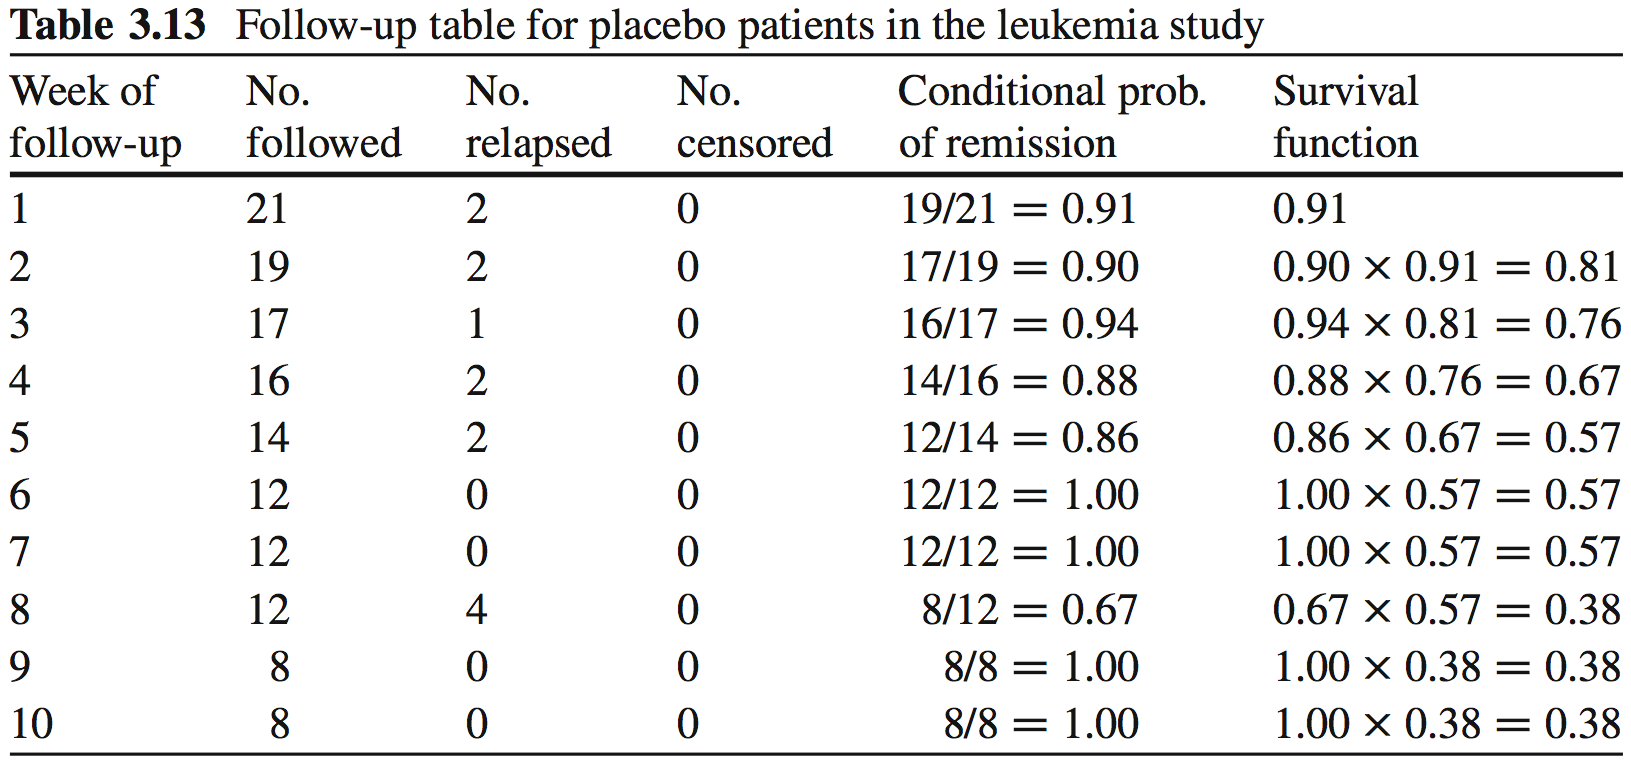
\includegraphics{figures/leukemiatable.png}
\caption{leukemia Follow-up Table}
\end{figure}

This is the \textbf{Kaplan-Meier Estimate} \(\hat S(t)\) of the Survival
function \(S(t)\).

\end{frame}

\begin{frame}[fragile]{Leukemia Kaplan-Meier plot}
\protect\hypertarget{leukemia-kaplan-meier-plot}{}

\begin{verbatim}
## Warning: Vectorized input to `element_text()` is not officially supported.
## Results may be unexpected or may change in future versions of ggplot2.
\end{verbatim}

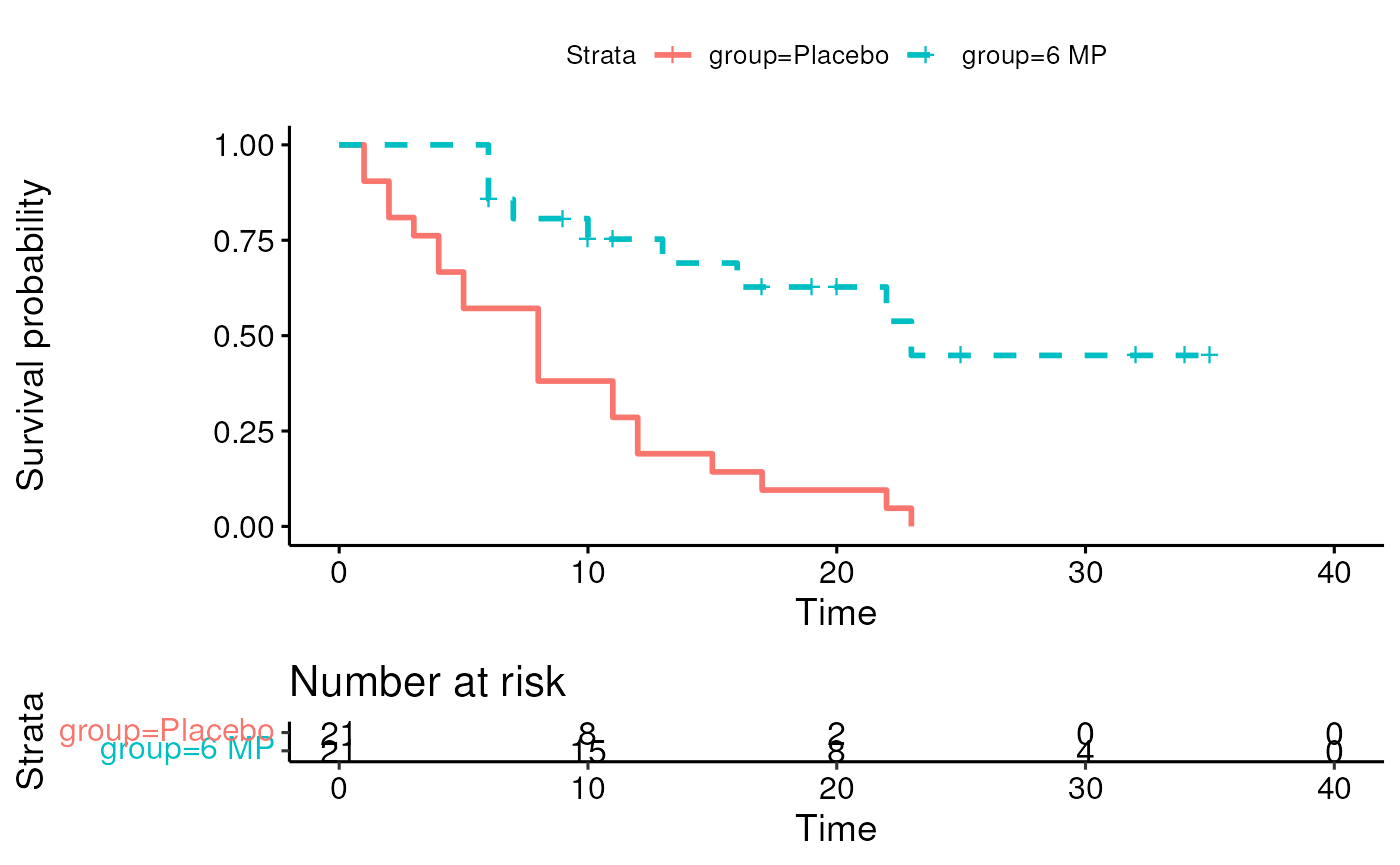
\includegraphics{../docs/articles/session_lecture_files/figure-beamer/unnamed-chunk-1-1.pdf}

\end{frame}

\begin{frame}{The hazard function h(t)}
\protect\hypertarget{the-hazard-function-ht}{}

\begin{itemize}
\item
  \emph{Definition}: The \emph{survival function} at time t, denoted
  \(S(t)\), is the probability of being event-free at t. Equivalently,
  it is the probability that the survival time is greater than t.
\item
  \emph{Definition}: The \emph{cumulative event function} at time t,
  denoted \(F(t)\), is the probability that the event has occurred by
  time t, or equivalently, the probability that the survival time is
  less than or equal to t. \(F(t) = 1-S(t)\).
\item
  \emph{Definition}: The \emph{hazard function} \(h(t)\) is the
  short-term event rate for subjects who have not yet experienced an
  event.

  \begin{itemize}
  \tightlist
  \item
    \(h(t)\) is the probability of an event in the time interval
    \([t, t+s]\) (s is small), given that the individual has survived up
    to time t
    \[h(t) = \lim_{s \to 0} \frac{Pr(t \leq T < t+s | T \ge t)}{s}\]
  \end{itemize}
\end{itemize}

\end{frame}

\begin{frame}{Leukemia dataset \(S(t)\)}
\protect\hypertarget{leukemia-dataset-st}{}

Survival function \(S(t)\)

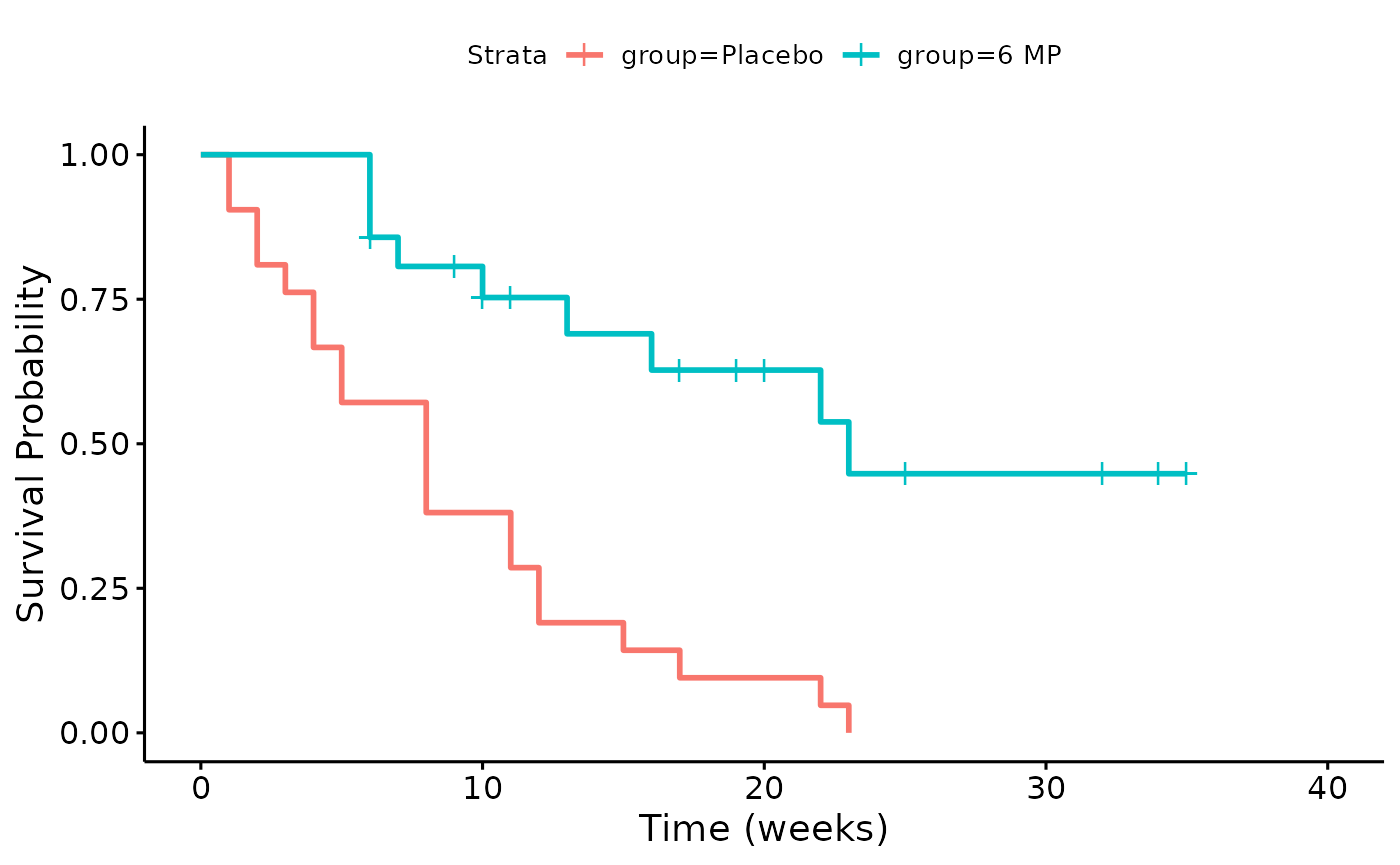
\includegraphics{../docs/articles/session_lecture_files/figure-beamer/unnamed-chunk-2-1.pdf}

\end{frame}

\begin{frame}{Leukemia dataset \(h(t)\)}
\protect\hypertarget{leukemia-dataset-ht}{}

Hazard function \(h(t)\)

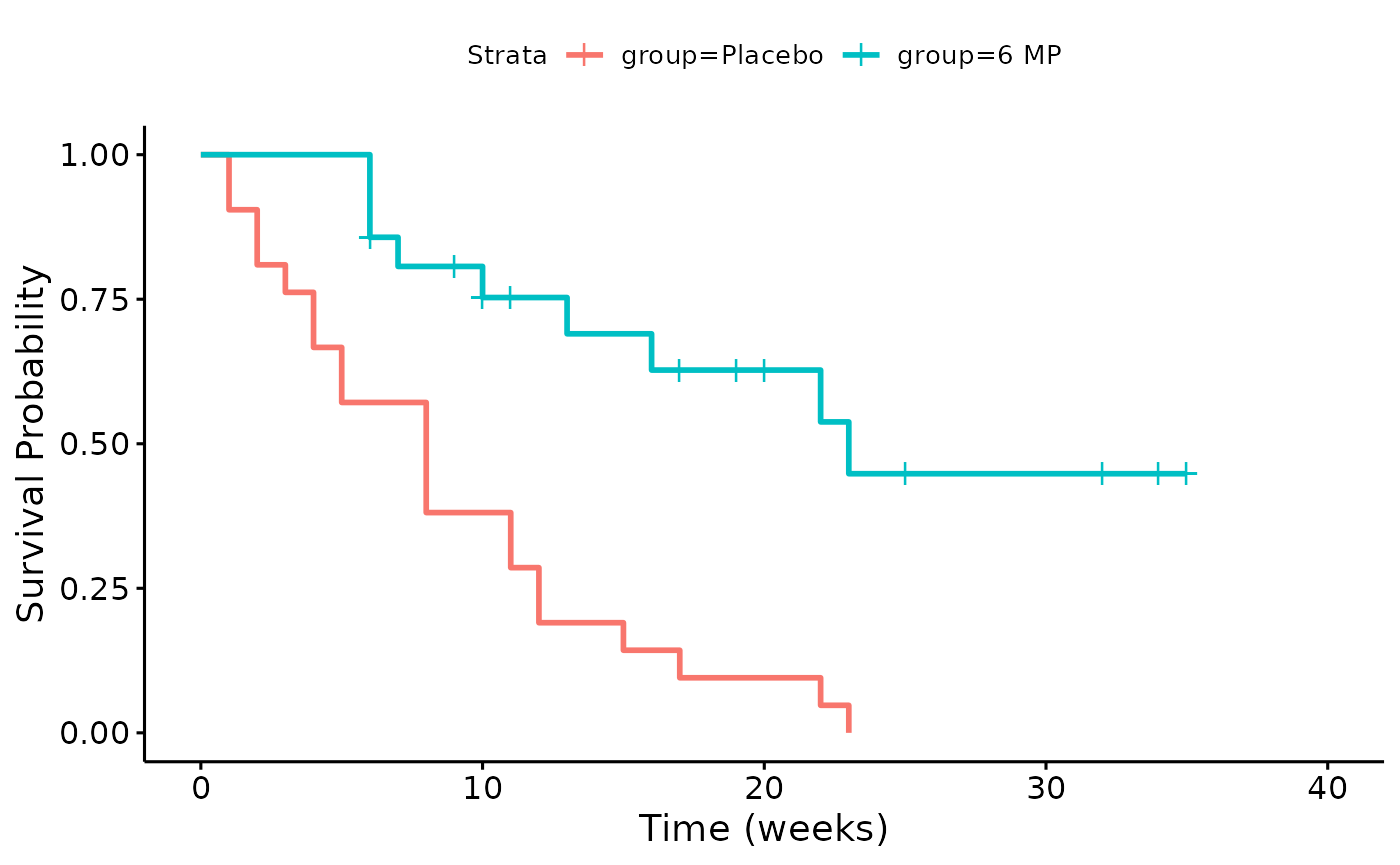
\includegraphics{../docs/articles/session_lecture_files/figure-beamer/unnamed-chunk-3-1.pdf}

\footnotesize

\href{http://sas-and-r.blogspot.com/2010/06/example-741-hazard-function-plotting.html}{SAS
and R Source code}

\end{frame}

\begin{frame}{The Hazard Ratio (HR)}
\protect\hypertarget{the-hazard-ratio-hr}{}

\begin{itemize}
\tightlist
\item
  If we are comparing the hazards of a control and a treatment group, it
  could in general be a function of time:

  \begin{itemize}
  \tightlist
  \item
    \(HR(t) = h_T(t) / h_C(t)\)
  \end{itemize}
\item
  Interpretation: the risk of event for the treatment group compared to
  the control group, as a function of time
\end{itemize}

\end{frame}

\begin{frame}{The Proportional Hazards Assumption}
\protect\hypertarget{the-proportional-hazards-assumption}{}

\begin{itemize}
\item
  \emph{Definition}: Under the \emph{proportional hazards assumption},
  the hazard ratio does not vary with time. That is,
  \(HR(t) \equiv HR\).
\item
  In other words, \(HR\) does not vary with time

  \begin{itemize}
  \tightlist
  \item
    \(HR(t)\) is a constant, \(HR\), at \emph{all times} t
  \item
    this assumption is about the population, of course there will be
    sampling variation
  \end{itemize}
\end{itemize}

\end{frame}

\begin{frame}{A nice proportional hazards dataset}
\protect\hypertarget{a-nice-proportional-hazards-dataset}{}

\begin{figure}
\centering
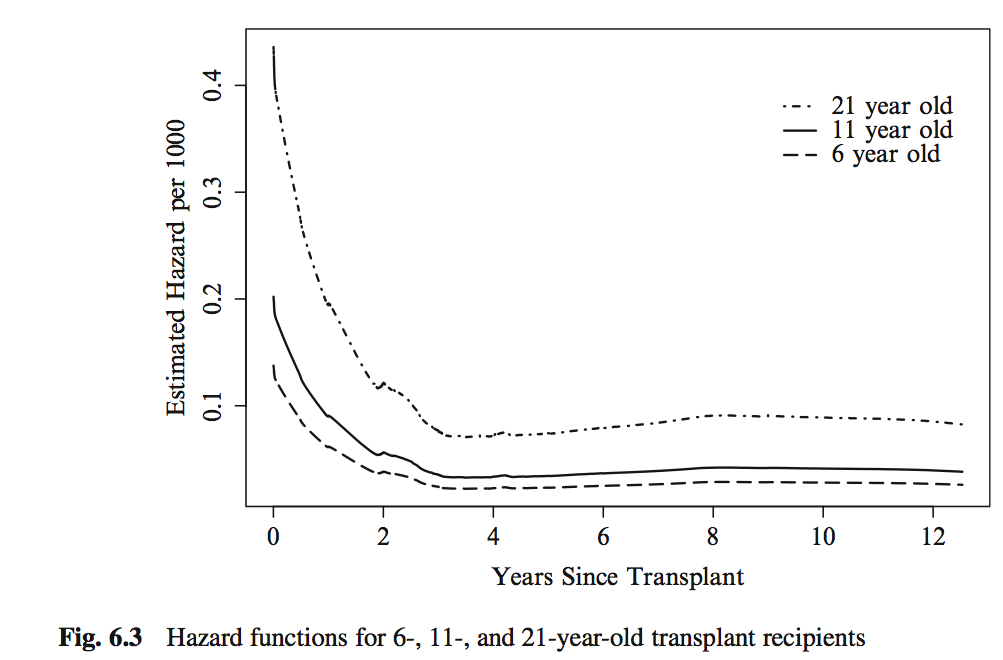
\includegraphics{figures/vittinghofffig63.png}
\caption{Vittinghoff Figure 6.3, p.~210}
\end{figure}

\end{frame}

\begin{frame}[fragile]{The hazard function h(t) (leukemia dataset)}
\protect\hypertarget{the-hazard-function-ht-leukemia-dataset}{}

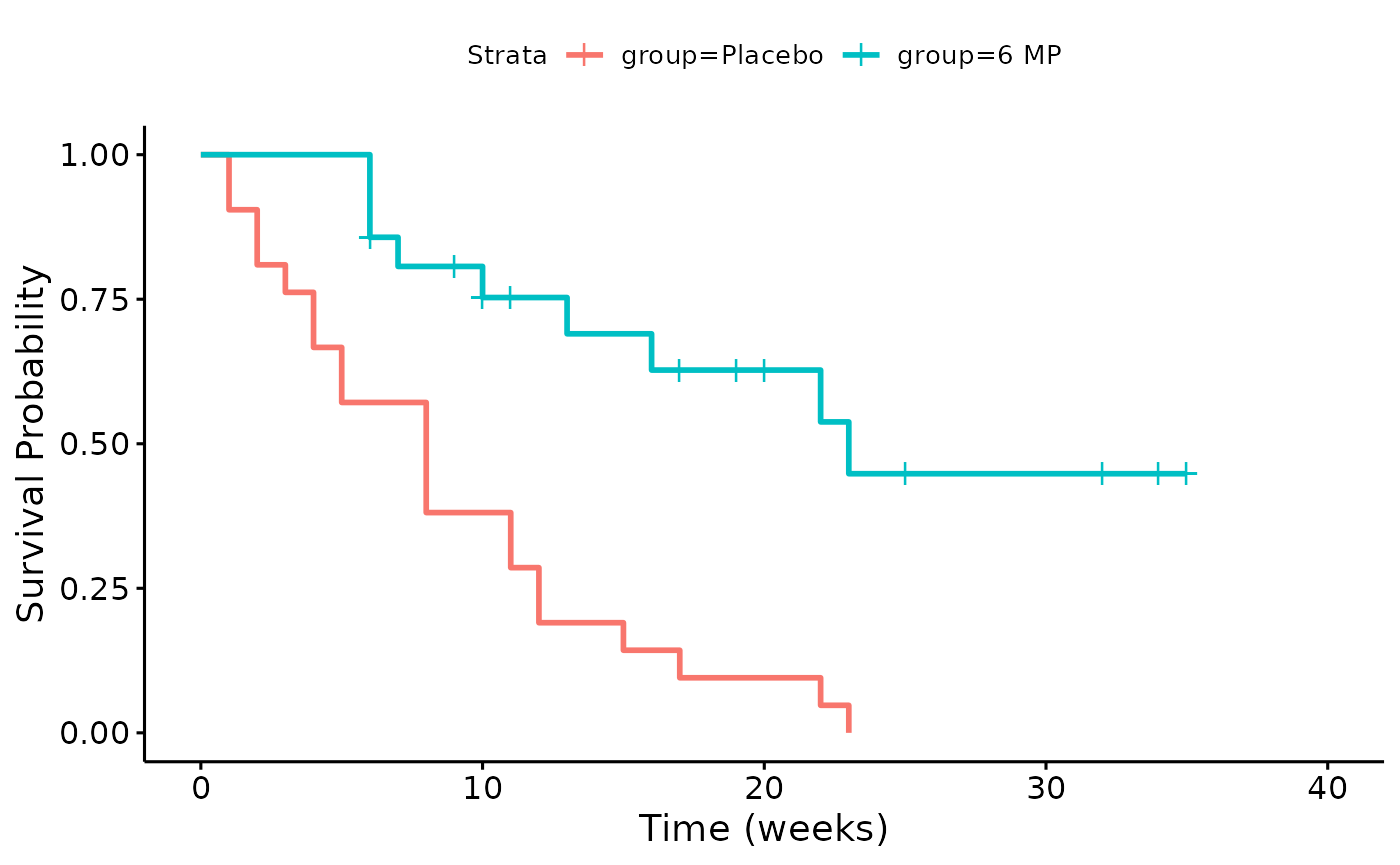
\includegraphics{../docs/articles/session_lecture_files/figure-beamer/unnamed-chunk-4-1.pdf}

\begin{verbatim}
## `summarise()` ungrouping output (override with `.groups` argument)
\end{verbatim}

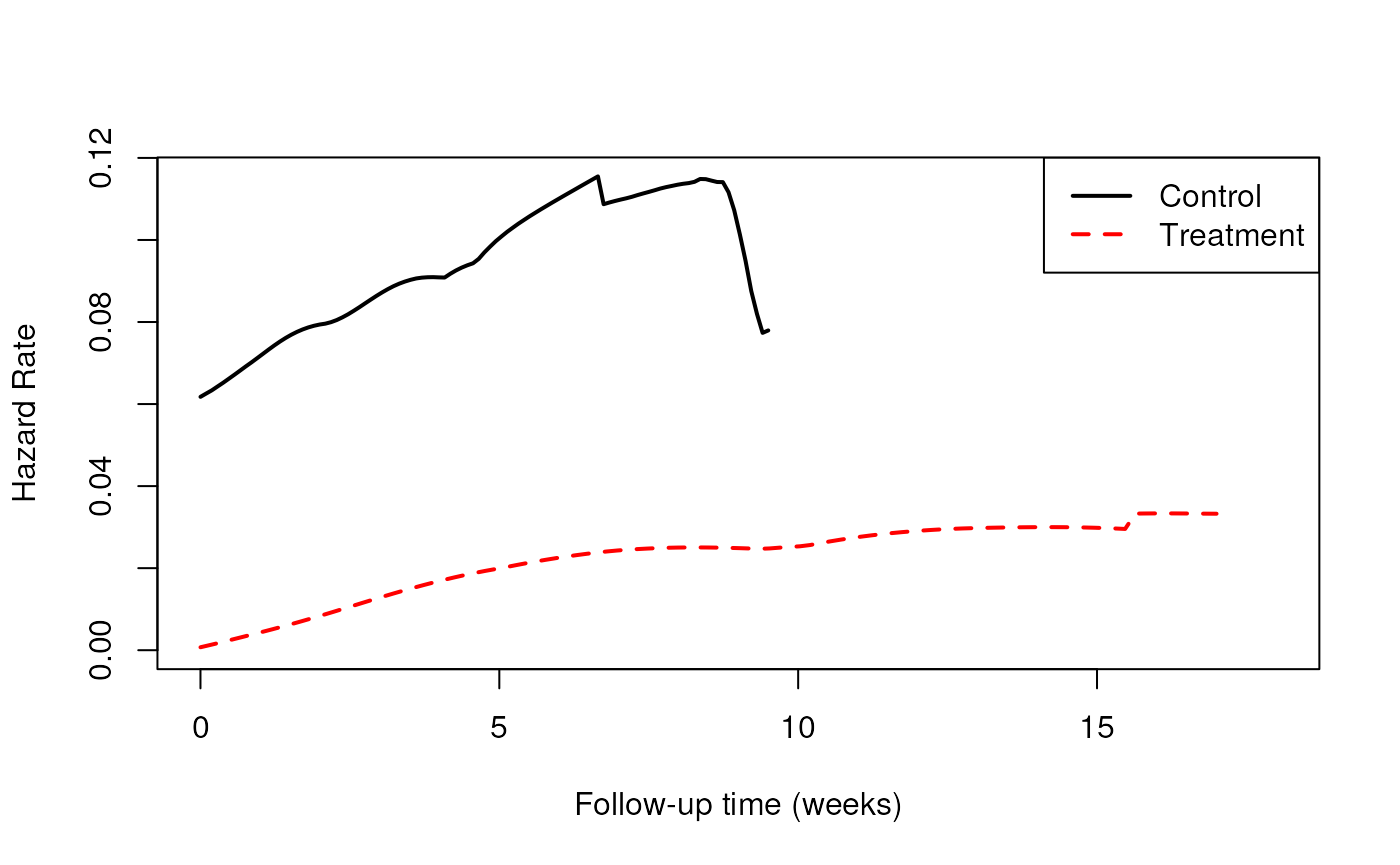
\includegraphics{../docs/articles/session_lecture_files/figure-beamer/unnamed-chunk-4-2.pdf}

\end{frame}

\begin{frame}{Log-minus-log plot}
\protect\hypertarget{log-minus-log-plot}{}

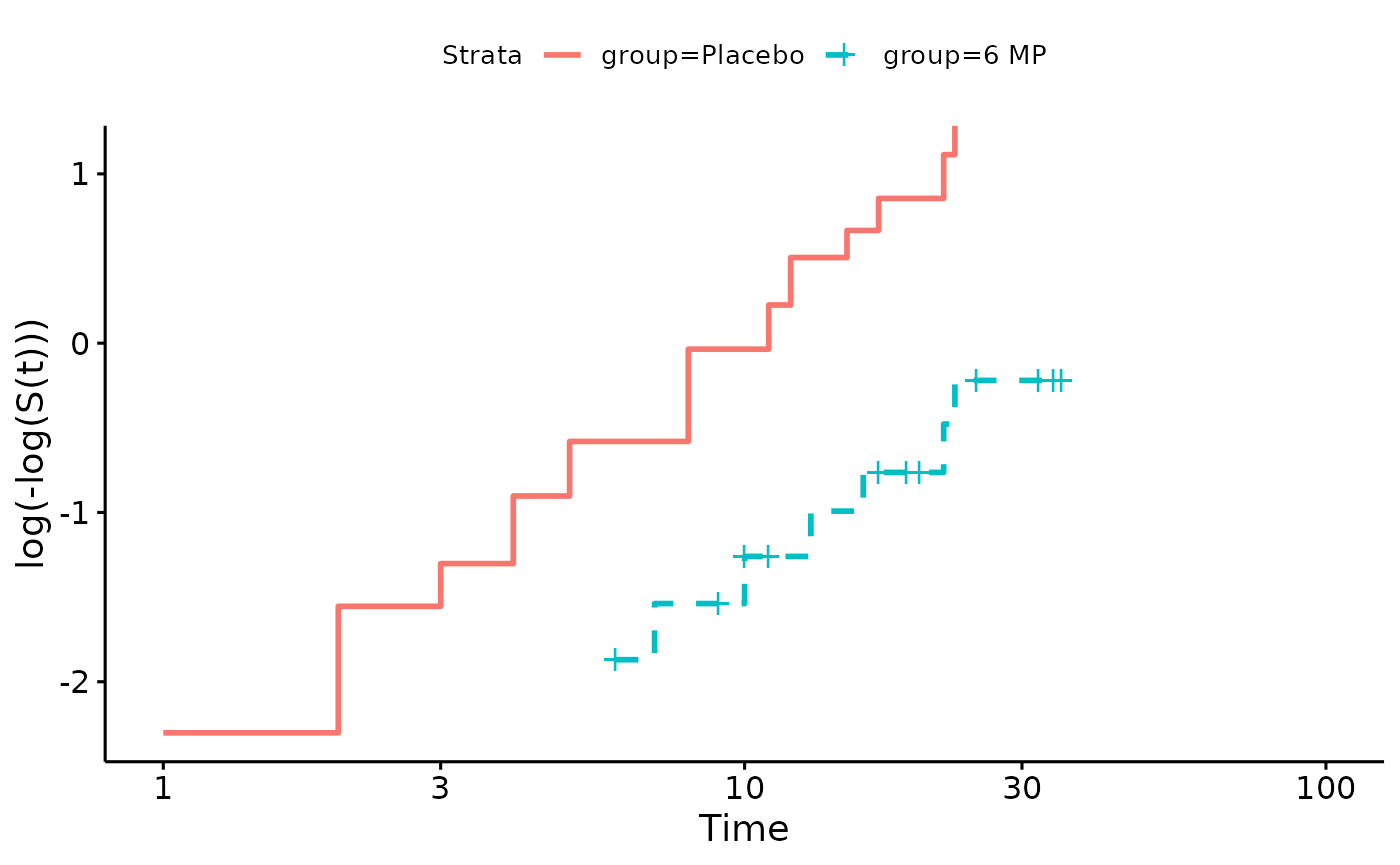
\includegraphics{../docs/articles/session_lecture_files/figure-beamer/unnamed-chunk-5-1.pdf}

\end{frame}

\begin{frame}{Recall previous regression models}
\protect\hypertarget{recall-previous-regression-models}{}

\[
E[y_i|x_i] = \beta_0 + \beta_1 x_{1i} + \beta_2 x_{2i} + ... + \beta_p x_{pi}
\]

\begin{itemize}
\tightlist
\item
  \(x_p\) are the predictors or independent variables
\item
  \(y\) is the outcome, response, or dependent variable
\item
  \(E[y|x]\) is the expected value of \(y\) given \(x\)
\item
  \(\beta_p\) are the regression coefficients
\end{itemize}

For logistic regression: \[
Logit(P(x_i)) = log \left( \frac{P(x_i)}{1-P(x_i)} \right) = \beta_0 + \beta_1 x_{1i} + \beta_2 x_{2i} + ... + \beta_p x_{pi}
\]

For log-linear regression: \[
log(E[y_i|x_i]) = \beta_0 + \beta_1 x_{1i} + \beta_2 x_{2i} + ... + \beta_p x_{pi}
\]

\end{frame}

\hypertarget{cox-proportional-hazards-model}{%
\section{Cox proportional hazards
model}\label{cox-proportional-hazards-model}}

\begin{frame}{Cox proportional hazards model}
\protect\hypertarget{cox-proportional-hazards-model-1}{}

\begin{itemize}
\tightlist
\item
  Cox proportional hazards regression assesses relationship between a
  right-censored, time-to-event outcome and predictors:

  \begin{itemize}
  \tightlist
  \item
    categorical variables (e.g., treatment groups)
  \item
    continuous variables \[
    log(HR(x_i)) = log \frac{h(t|x_i)}{h_0(t)} = \beta_0 + \beta_1 x_{1i} + \beta_2 x_{2i} + ... + \beta_p x_{pi}
    \]
  \end{itemize}
\item
  \(HR(x_i)\) is the hazard of patient \(i\) relative to baseline
\item
  \(h(t|x_i)\) is the time-dependent hazard function \(h(t)\) for
  patient \(i\)
\item
  \(h_0(t)\) is the \emph{baseline hazard function}
\end{itemize}

Multiplicative or additive model?

\end{frame}

\begin{frame}{Interpretation of coefficients}
\protect\hypertarget{interpretation-of-coefficients}{}

\begin{itemize}
\tightlist
\item
  Coefficients \(\beta\) for a categorical / binary predictor:

  \begin{itemize}
  \tightlist
  \item
    \(\beta\) is the \(log\) of the ratio of hazards for the comparison
    group relative to reference group (\(log(HR)\))
  \end{itemize}
\item
  Coefficients \(\beta\) for a continuous predictor:

  \begin{itemize}
  \tightlist
  \item
    \(\beta\) is the \(log\) of the ratio of hazards for someone having
    a one unit higher value of \(x\) (1 year, 1mm Hg, etc)
  \end{itemize}
\item
  If the hazard ratio (\(exp(\beta)\)) is close to 1 then the predictor
  does not affect survival
\item
  If the hazard ratio is less than 1 then the predictor is protective
  (associated with improved survival)
\item
  If the hazard ratio is greater than 1 then the predictor is associated
  with increased risk (= decreased survival)
\end{itemize}

\end{frame}

\begin{frame}{Hypothesis testing and CIs}
\protect\hypertarget{hypothesis-testing-and-cis}{}

\begin{itemize}
\tightlist
\item
  Wald Test or Likelihood Ratio Test for coefficients

  \begin{itemize}
  \tightlist
  \item
    \(H_0: \beta=0, H_a: \beta \neq 0\)
  \item
    equivalent to \(H_0: HR=1, H_a: HR \neq 1\)
  \end{itemize}
\item
  CIs typically obtained from Wald Test, reported for \(HR\)
\end{itemize}

\end{frame}

\begin{frame}[fragile]{CoxPH regression for Leukemia dataset}
\protect\hypertarget{coxph-regression-for-leukemia-dataset}{}

\tiny

\begin{verbatim}
## Call:
## coxph(formula = Surv(time, cens) ~ group, data = leuk)
## 
##   n= 42, number of events= 30 
## 
##              coef exp(coef) se(coef)      z Pr(>|z|)    
## group6 MP -1.5721    0.2076   0.4124 -3.812 0.000138 ***
## ---
## Signif. codes:  0 '***' 0.001 '**' 0.01 '*' 0.05 '.' 0.1 ' ' 1
## 
##           exp(coef) exp(-coef) lower .95 upper .95
## group6 MP    0.2076      4.817   0.09251    0.4659
## 
## Concordance= 0.69  (se = 0.041 )
## Likelihood ratio test= 16.35  on 1 df,   p=5e-05
## Wald test            = 14.53  on 1 df,   p=1e-04
## Score (logrank) test = 17.25  on 1 df,   p=3e-05
\end{verbatim}

\end{frame}

\begin{frame}{Cox PH is a semi-parametric model}
\protect\hypertarget{cox-ph-is-a-semi-parametric-model}{}

\begin{itemize}
\tightlist
\item
  Cox proportional hazards model is \emph{semi-parametric}:

  \begin{itemize}
  \tightlist
  \item
    assumes proportional hazards (PH), but no assumption on \(h_0(t)\)
  \item
    robust if PH assumption is not violated
  \item
    time-dependent covariates may resolve apparent violations of the PH
    assumption.
  \end{itemize}
\end{itemize}

\end{frame}

\begin{frame}{Summary: proportional hazards assumption}
\protect\hypertarget{summary-proportional-hazards-assumption}{}

\begin{itemize}
\tightlist
\item
  Constant hazard \emph{ratio} between groups over time (proportional
  hazards)
\item
  A linear association between the natural log of the relative hazard
  and the predictors (log-linearity)

  \begin{itemize}
  \tightlist
  \item
    A multiplicative relationship between the predictors and the hazard
  \end{itemize}
\item
  Uninformative censoring
\end{itemize}

\end{frame}

\begin{frame}{What to do when proportional hazards doesn't hold?}
\protect\hypertarget{what-to-do-when-proportional-hazards-doesnt-hold}{}

\begin{itemize}
\tightlist
\item
  \textbf{Time-dependent covariates}
\item
  \textbf{Definition}: A time-dependent covariate is a predictor whose
  values may vary with time.
\item
  \textbf{Basic rule}: You cannot look into the future in your analysis
  (even though it took place in the past) E.g.:

  \begin{itemize}
  \tightlist
  \item
    breast cancer chemotherapy patients divided into groups based on how
    much of the planned dose they received
  \item
    patients divided into groups based on early response to treatment
    (shrinkage of tumor, lowering of cholesterol, etc)
  \item
    interpolation of the values of a laboratory test linearly between
    observation times
  \item
    removing subjects who do not finish the treatment plan
  \item
    imputing the date of an adverse event as midway between observation
    times
  \end{itemize}
\end{itemize}

Source:
\href{https://cran.r-project.org/web/packages/survival/vignettes/timedep.pdf}{Using
Time Dependent Covariates and Time Dependent Coefficients in the Cox
Model}

\end{frame}

\begin{frame}{Immortal time bias example}
\protect\hypertarget{immortal-time-bias-example}{}

\begin{itemize}
\tightlist
\item
  Immortal time bias is an example of looking into the future.
\item
  E.g. Yee \emph{et al.} reported that new statin users reported a 26\%
  reduction in the risk of diabetes progression with one year or more of
  treatment relative to never-users (adjusted HR 0.74, 95\% CI: 0.56 to
  0.97).

  \begin{itemize}
  \tightlist
  \item
    New users excludes those who had received a lipid lowering drug from
    three years before to six months after cohort entry
  \end{itemize}
\item
  This is a surprising finding because of confounding: people whose
  diabetes progresses are more likely to develop cardiovascular disease,
  an indication for statins.

  \begin{itemize}
  \tightlist
  \item
    would result in HR \textgreater{} 1
  \end{itemize}
\item
  This is a result of an analysis error. Why?
\end{itemize}

\tiny

\begin{itemize}
\tightlist
\item
  Yee \emph{et al.} Statin use in type 2 diabetes mellitus is associated
  with a delay in starting insulin
  (\url{http://onlinelibrary.wiley.com/doi/10.1111/j.1464-5491.2004.01263.x/full})
\end{itemize}

\end{frame}

\begin{frame}{Immortal time bias example (cont'd)}
\protect\hypertarget{immortal-time-bias-example-contd}{}

\begin{itemize}
\tightlist
\item
  What was the analysis error?

  \begin{itemize}
  \tightlist
  \item
    all person days between cohort entry and end of follow-up were
    \textbf{classified as treated} for those who met the statin user
    definition, regardless of the date on which they met this definition
    and as untreated for non-users
  \item
    thus all persons in the \emph{treated} group are ``immortal'' from
    time 0 until the initiation of statin treatment
  \item
    this period of immortality makes treatment look more effective
  \end{itemize}
\end{itemize}

\end{frame}

\hypertarget{parametric-survival-models}{%
\section{Parametric survival models}\label{parametric-survival-models}}

\begin{frame}{What are ``parametric'' survival models?}
\protect\hypertarget{what-are-parametric-survival-models}{}

\begin{itemize}
\tightlist
\item
  ``Parametric'' models estimate additional \emph{parameters} for the
  baseline hazard, e.g.:

  \begin{itemize}
  \tightlist
  \item
    \textbf{Weibull}: hazard function is a polynomial
  \item
    \textbf{exponential}: hazard function is constant over time,
    survival function is exponential (special case of Weibull):
    e.g.~healthy population with randomly occurring events
  \item
    many other options for assumption of distributions
  \end{itemize}
\item
  In most common implementation a log-transform of the time variable is
  used

  \begin{itemize}
  \tightlist
  \item
    then can be interpreted as \emph{Accelerated Failure Time} (AFT)
    models.
  \end{itemize}
\end{itemize}

\end{frame}

\begin{frame}{Coefficients in parametric models}
\protect\hypertarget{coefficients-in-parametric-models}{}

\begin{itemize}
\tightlist
\item
  The interpretation of \(\beta\) coefficients is different:

  \begin{itemize}
  \tightlist
  \item
    Cox model: \(log(HR)\)
  \item
    AFT models: \(log(survival time ratio)\)
  \item
    The sign is \emph{opposite} (\emph{i.e.} if one is positive the
    other is negative)
  \end{itemize}
\end{itemize}

\end{frame}

\begin{frame}[fragile]{Why use a parametric survival model?}
\protect\hypertarget{why-use-a-parametric-survival-model}{}

\begin{itemize}
\tightlist
\item
  Can be more powerful if assumption is correct

  \begin{itemize}
  \tightlist
  \item
    may help with small numbers of events
  \end{itemize}
\item
  Extra capabilities:

  \begin{itemize}
  \tightlist
  \item
    smooth estimation of baseline hazard
  \item
    extrapolation
  \item
    complicated censoring
  \end{itemize}
\item
  Easy to interpret: coefficients are \(log(survival time ratio)\)
\item
  Easy to fit: replace \texttt{survival::coxph} with
  \texttt{survival::survreg}
\end{itemize}

\end{frame}

\begin{frame}{Why not to use a parametric survival model?}
\protect\hypertarget{why-not-to-use-a-parametric-survival-model}{}

\begin{itemize}
\tightlist
\item
  Depend on correct specification of baseline hazard model
\item
  Even if correctly specified, may not provide much improvement in
  efficiency
\item
  Still make a proportionality assumption, on survival functions
\end{itemize}

\end{frame}

\end{document}
